% Chapter Chapter 7 For Reproducible Research in R and RStudio
% Christopher Gandrud
% Created: 16/07/2012 05:45:03 pm CEST
% Updated: 28 December 2012




\chapter{Preparing Data for Analysis}\label{DataClean}

Once we have gathered the raw data that we want to include in our statistical analyses we generally need to clean so that it can be merged it into a single data file. This chapter covers some of the basics of how to clean data files and merge them together into one data frame using R. If you are very familiar with data transformations in R you may want to skip onto the next chapter. 

\section{Cleaning data for merging}

In order to successfully merge two or more data frames we need to make sure that they are in the same format. Let's look at some of the important formatting issues and how to reformat your data frames so that they can be easily merged.

\subsection{Get a handle on your data}

Before doing anything to your data it is a good idea to take a look at it and see what needs to be done. Surprisingly, just taking a little time to look at your data will help you avoid many error messages and much frustration. 

To get a sense of your data you could of course just type a data frame object's name into the R console. This will print the entire data frame. For data frames with more than a few variables and observations. We have already seen a number of commands that are useful for seeing parts of your data. The \texttt{names}\index{names} command shows you the variable names of a data frame object. The \texttt{head}\index{head} command shows the first few observations in a data frame and \texttt{tail}\index{tail} shows the last few.

The \texttt{summary} command\index{summary, R command} is especially helpful for seeing not only basic descriptive statistics for all of the variables in a data frame, but also the variables' types. For example, let's us the \emph{AgMethaneData} object we created in Chapter \ref{DataGather}:

{\small
\begin{knitrout}
\definecolor{shadecolor}{rgb}{0.969, 0.969, 0.969}\color{fgcolor}\begin{kframe}
\begin{alltt}
\hlcomment{# Summarize AgMethaneData data frame object}
\hlfunctioncall{summary}(AgMethaneData)
\end{alltt}
\begin{verbatim}
##     iso2c             country          EN.ATM.METH.AG.ZS      year     
##  Length:984         Length:984         Min.   : 0.0      Min.   :2002  
##  Class :character   Class :character   1st Qu.:27.7      1st Qu.:2003  
##  Mode  :character   Mode  :character   Median :43.3      Median :2004  
##                                        Mean   :43.4      Mean   :2004  
##                                        3rd Qu.:61.8      3rd Qu.:2004  
##                                        Max.   :93.4      Max.   :2005  
##                                        NA's   :820
\end{verbatim}
\end{kframe}
\end{knitrout}

}

\noindent We can immediately see that the variables \textbf{iso2C} are character strings. Because \emph{summary} is able to calculate means, medians, and so on for \textbf{EN.ATM.METH.AG.ZS} and \textbf{year} we know they are numeric. You can of course run \emph{summary} on a particular variable by using the component selector (\verb|$|):

\begin{knitrout}
\definecolor{shadecolor}{rgb}{0.969, 0.969, 0.969}\color{fgcolor}\begin{kframe}
\begin{alltt}
\hlcomment{# Summarize the methane emissions variable from AgMethaneData}
\hlfunctioncall{summary}(AgMethaneData$EN.ATM.METH.AG.ZS)
\end{alltt}
\begin{verbatim}
##    Min. 1st Qu.  Median    Mean 3rd Qu.    Max.    NA's 
##     0.0    27.7    43.3    43.4    61.8    93.4     820
\end{verbatim}
\end{kframe}
\end{knitrout}


\noindent We'll come back to why knowing this type of information is important for merging and data analysis later in this Chapter.

If you are using R in the Terminal or the R GUI program you can view a portion of a data frame object with the \texttt{View} command.\index{View R command} This will open a new window that lets you see a selection of the data frame. For example, \verb|View(AgMethaneData)| will give you the window shown in the left-hand pane in Figure \ref{ViewerFig}. If you are using RStudio, you can click on the data frame in the \emph{Workspace} tab and you will get something that looks like the right-hand panel in Figure \ref{ViewerFig}.

{\small
\begin{figure}
	\caption{R Data Viewers}
	\label{ViewerFig}
	\centering
		\begin{minipage}[b]{0.5\textwidth}
			\centering
  			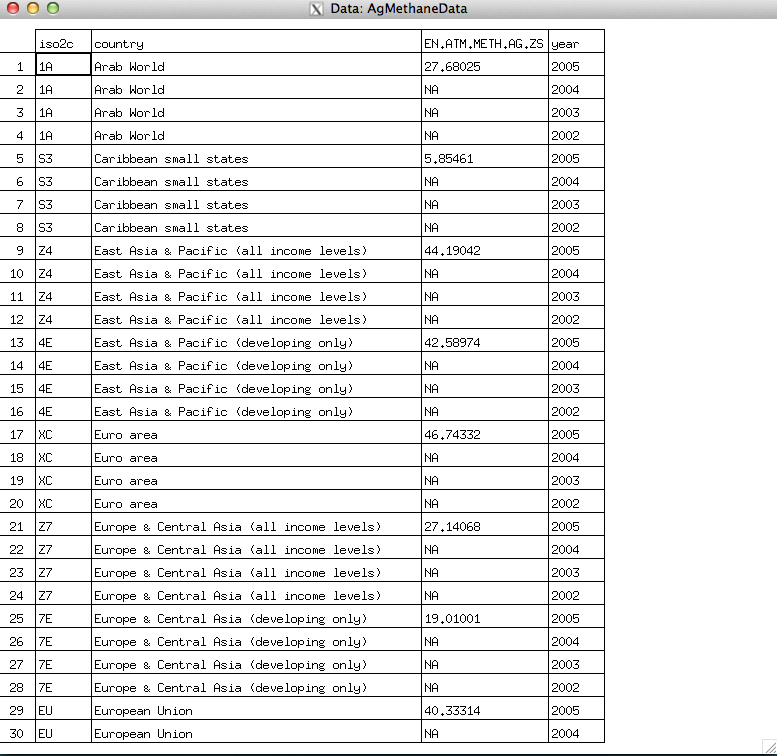
\includegraphics[width=.45\linewidth]{/git_repositories/Rep-Res-Book/Source/Children/Chapter7/images7/ViewerX11.png}
  			\caption{Viewer for Terminal/R GUI}
  		\end{minipage}

  		\hfill

 		\begin{minipage}[b]{0.5\textwidth}
  			\centering
  			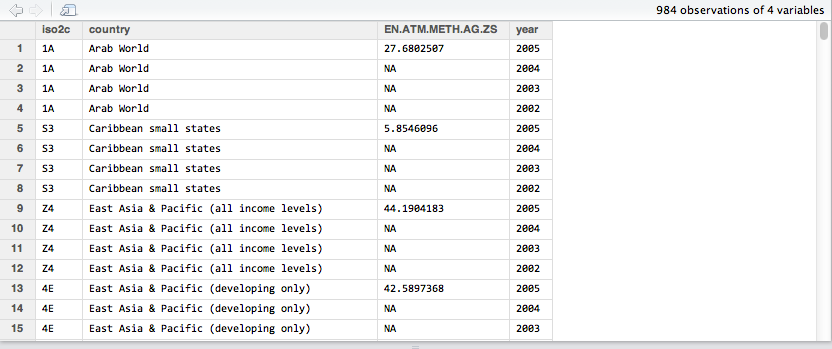
\includegraphics[width=.45\linewidth]{/git_repositories/Rep-Res-Book/Source/Children/Chapter7/images7/ViewerRStudio.png}
  			\caption{Viewer for RStudio}
  		\end{minipage}
\end{figure}
}
\noindent Note that neither of these viewers are interactive in that you can't use them to manipulate the data. They are only data viewers.

\subsection{Reshaping Data}

Obviously it is usually a good if the data sets kept in data frame type objects. See Chapter \ref{GettingStartedRKnitr} (page \pageref{data.frame}) for how to convert objects into data frames with the \texttt{data.frame} command. Not only do data sets (generally) need to be stored in data frame objects they also need to follow the same layout. Most R statistical analysis tools assume that your data is in ``long'' format\index{long formatted data} (as we also did in Chapter \ref{GettingStartedRKnitr}). This means that data frame columns are variables and rows are observations (see Table \ref{ExampleLong}).

\begin{table}[h!]
	\caption{Long Formatted Data Example}
	\label{ExampleLong}
	\begin{tabular}{l c c c}
		\hline
		Observation & Variable1 & Variable2 & \ldots \\
		\hline \\[0.1cm]
		Subject1 & & & \\[0.25cm]
		Subject2 & & & \\[0.25cm]
		Subject3 & & & \\[0.25cm]
		\ldots & & & \\[0.25cm]
		\hline
	\end{tabular}
\end{table}

\noindent If one of your data sets is not in this format then you will need to reshape\index{reshape data} it. Some data sets are in ``wide'' format;\index{wide formatted data} where the columns (apart from the first one) are observations and the rows are variables (see Table \ref{ExampleWide}).

\begin{table}[h!]
	\caption{Wide Formatted Data Example}
	\label{ExampleWide}
	\begin{tabular}{l c c c}
		\hline 
		Variables & Subject1 & Subject2 & \ldots \\
		\hline \\[0.1cm]
		Variable1 & & & \\[0.25cm]
		Variable2 & & & \\[0.25cm]
		Variable3 & & & \\[0.25cm]
		\ldots & & & \\[0.25cm]
		\hline
	\end{tabular}
\end{table}

There are  has a number of very useful functions for changing data from wide format to long and vice versa. Lets look first at the matrix transpose function (\texttt{t}). Imagine we have the following data:




\begin{knitrout}
\definecolor{shadecolor}{rgb}{0.969, 0.969, 0.969}\color{fgcolor}\begin{kframe}
\begin{alltt}
WidePop
\end{alltt}
\begin{verbatim}
##     variable Albania Botswana Cambodia
## 1 population     2.8      2.0     14.8
\end{verbatim}
\end{kframe}
\end{knitrout}


\noindent What we really want is a data frame with the observations (countries) as the rows and the \textbf{population} variable in a column. If we run \emph{WidePop} through the matrix transpose function we will get:

\begin{knitrout}
\definecolor{shadecolor}{rgb}{0.969, 0.969, 0.969}\color{fgcolor}\begin{kframe}
\begin{alltt}
\hlcomment{# Matrix transpose WidePop}
LongPop <- \hlfunctioncall{t}(WidePop)

\hlcomment{# Show LongPop}
LongPop
\end{alltt}
\begin{verbatim}
##          [,1]        
## variable "population"
## Albania  "2.8"       
## Botswana "2.0"       
## Cambodia "14.8"
\end{verbatim}
\end{kframe}
\end{knitrout}


\noindent We need to clean up \emph{LongPop} a little bit before it is ready to use. The first thing is to change \emph{LongPop} back into a data frame.


